\begin{frame}{$\chi_{b1,2}(3P) \to \ThreeS \gamma$ fit model}
\begin{columns}[T]
\column{.5\textwidth}
  \centering
  \setlength{\unitlength}{1mm}
  \begin{picture}(50,80)
      %
    \put(0,0){
      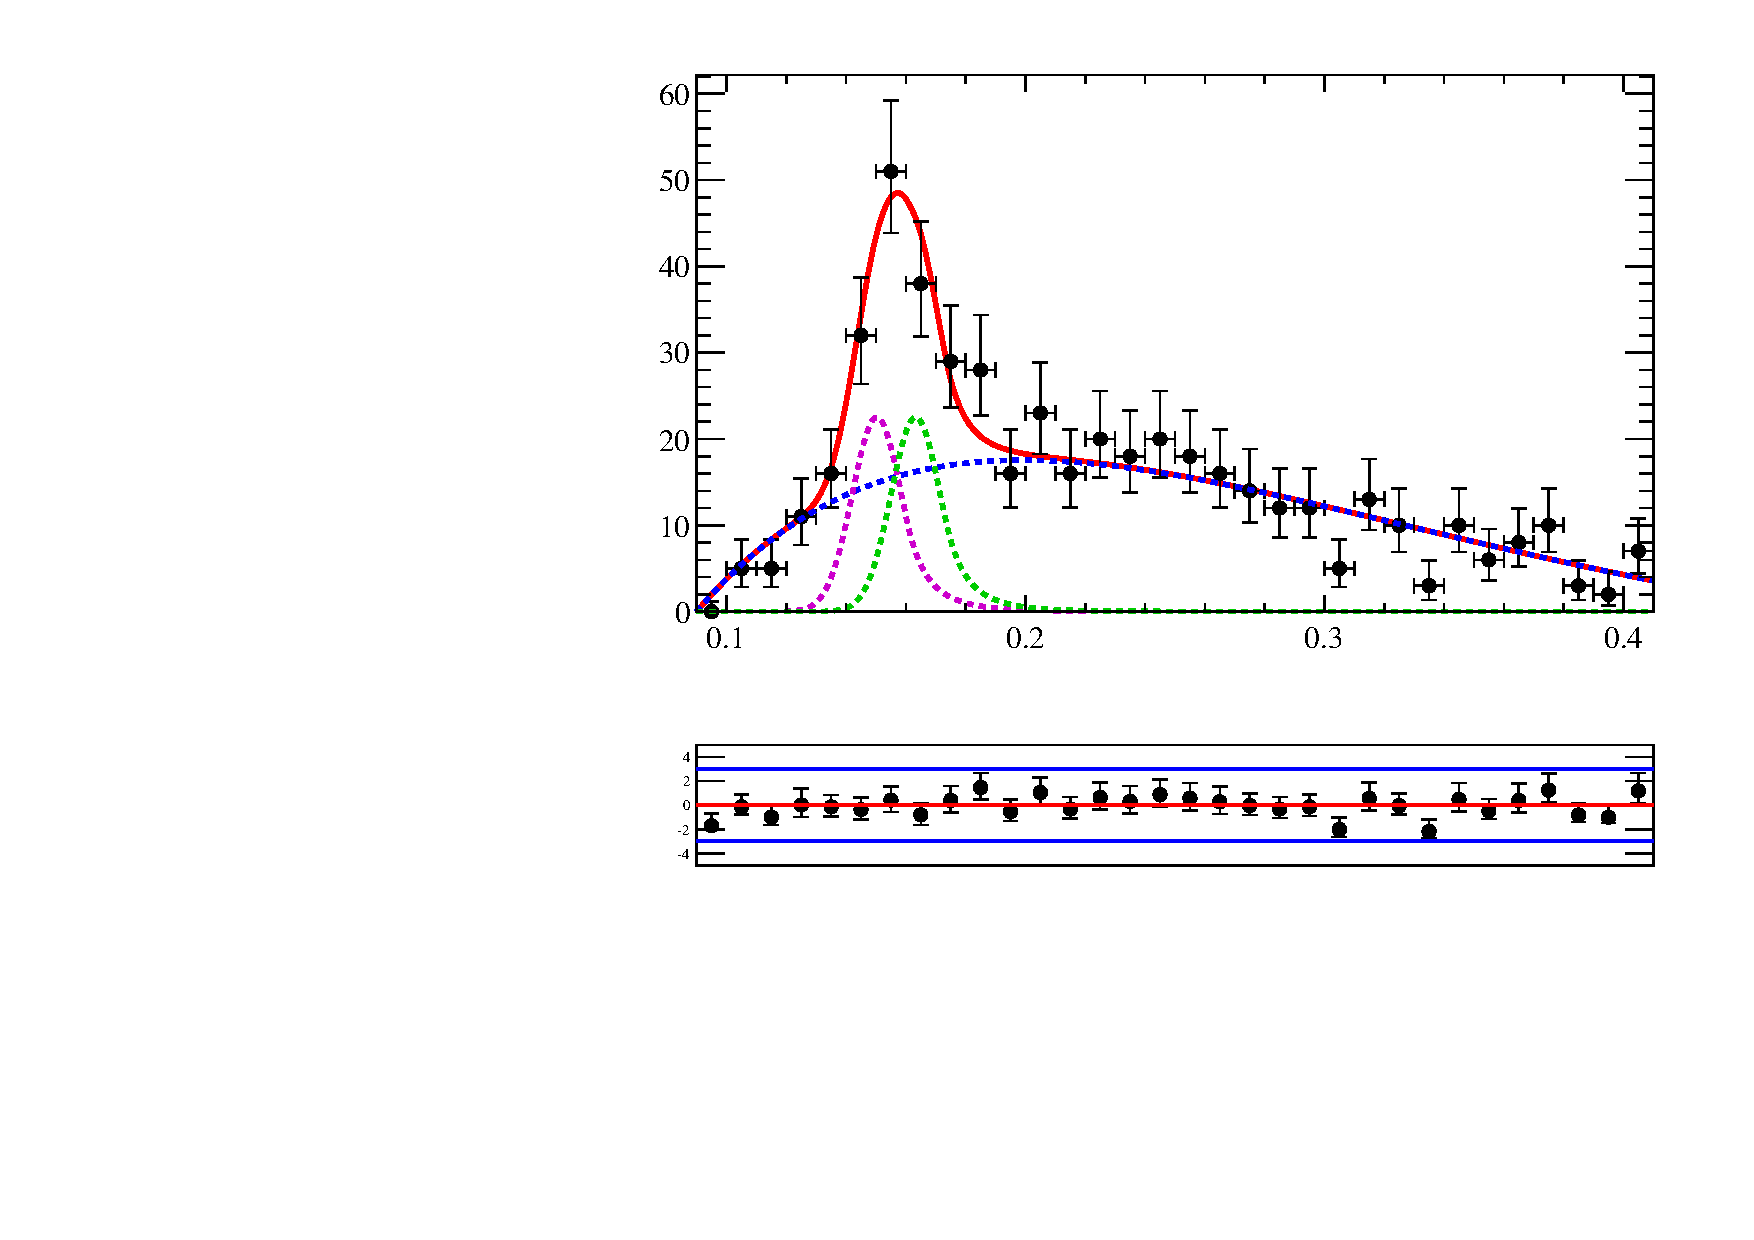
\includegraphics[width=50mm, height=40mm]{chib3s-fit/f2012_27_40}
    }
    
    \put(0,40){
      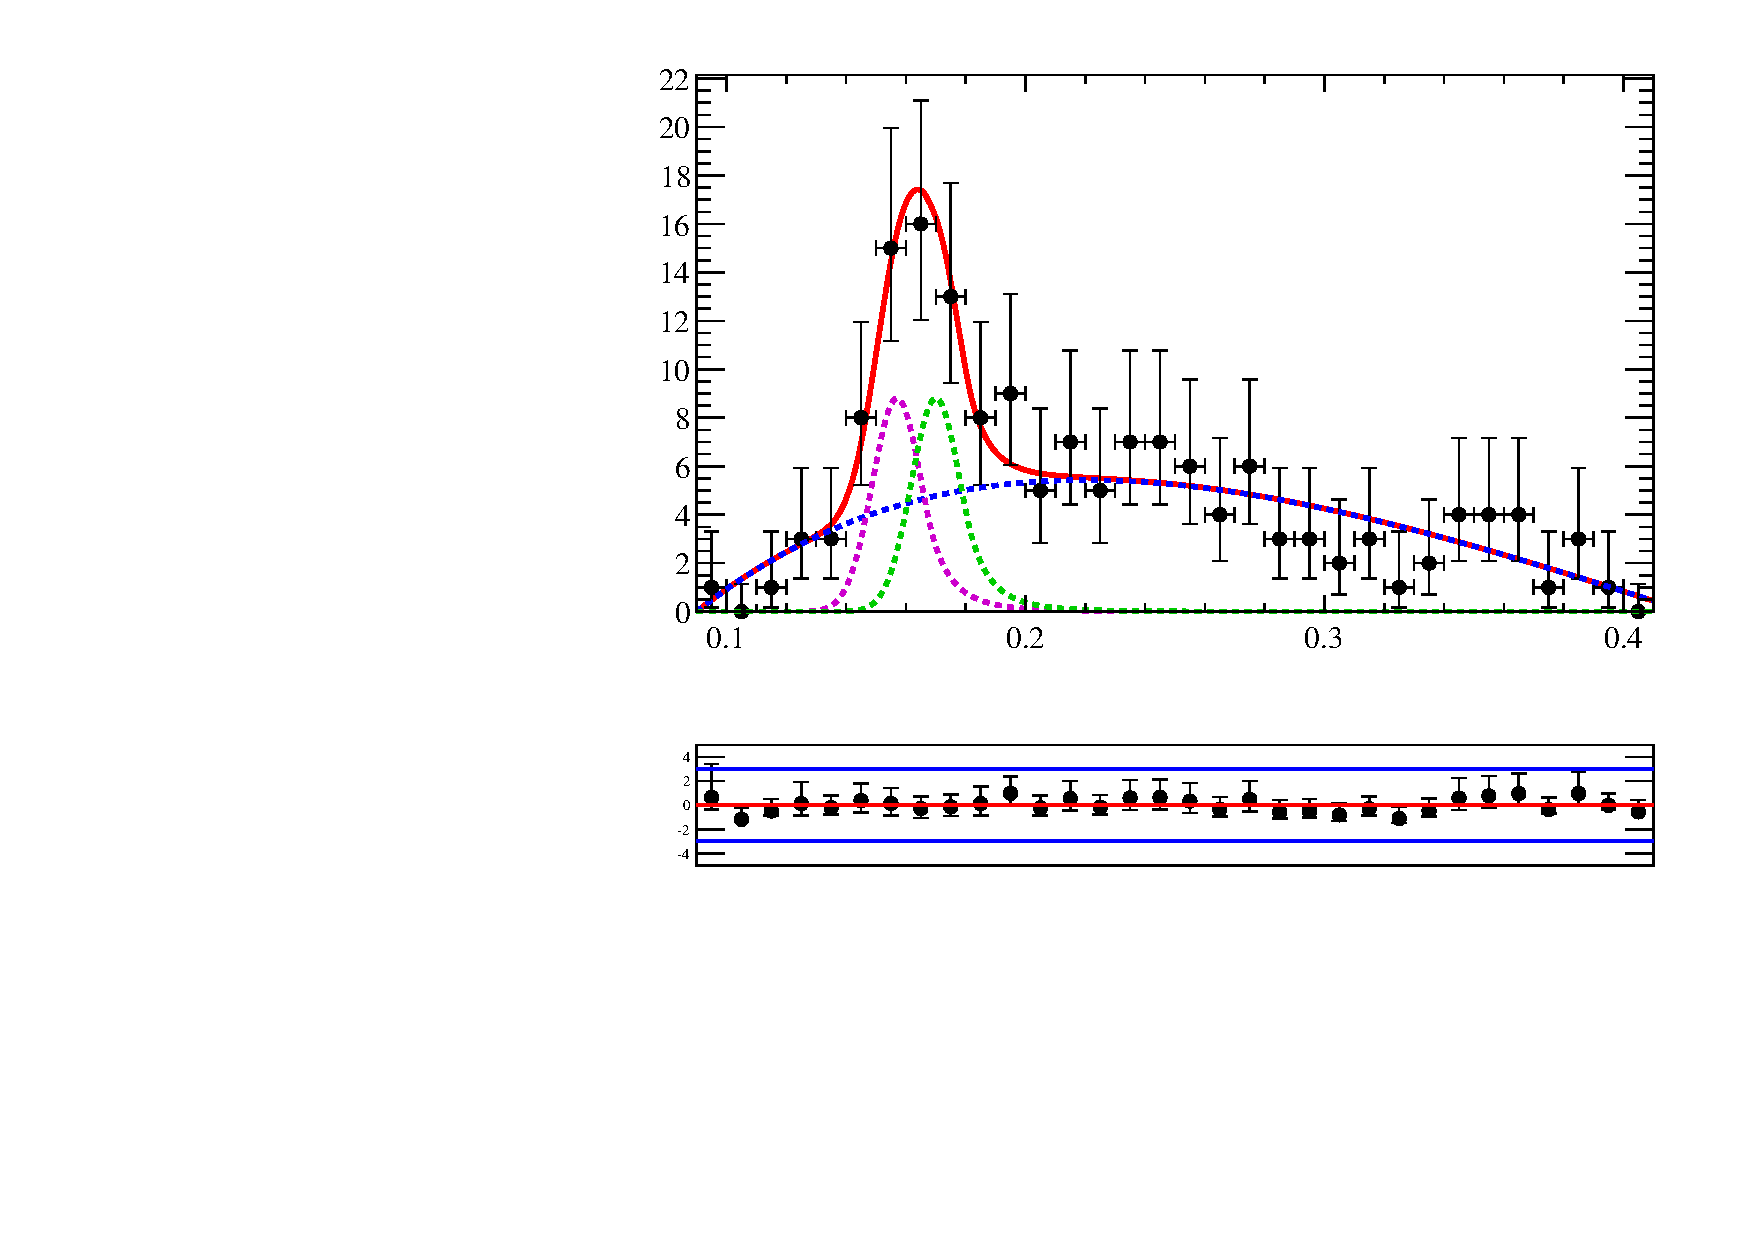
\includegraphics[width=50mm, height=40mm]{chib3s-fit/f2011_27_40}
    }

    \put(0,15){\tiny \begin{sideways}Candidates/(20\mevcc)\end{sideways}}
    \put(2,9){\tiny $m_{\mumu \gamma} - m_{\mumu} + m_{\Y3S}^{PDG} \left[\gevcc\right]$}
    \put(25,30){$\sqs=8\gev$}
    \put(20,25){\tiny $27 < p_T^{\Y3S} <  40 \gevc$}    
    
    \put(0,55){\tiny \begin{sideways}Candidates/(20\mevcc)\end{sideways}}
    \put(2, 49){\tiny $m_{\mumu \gamma} - m_{\mumu} + m_{\Y3S}^{PDG} \left[\gevcc\right]$}
    \put(25,70){$\sqs=7\gev$}     
    \put(20,65){\tiny $27 < p_T^{\Y3S} <  40 \gevc$}        
    
    \put(10,75){\tiny \chibThreeP}
    \put(10,35){\tiny \chibThreeP}

    % \graphpaper[5](0,0)(50, 80)        
  \end{picture}
\column{.5\textwidth}
\begin{itemize}
\item One Crystal Ball (CB) for each $\chi_{b1,2}(3P)$ state: 2 CB in total
\item Exclude the study of $\chi_{b0}$ due to its low radiative branching ratio.
\item Product of exponential and linear combination of polynomials  for combinatorial background.
\end{itemize}
\end{columns}
\end{frame}
